Non esistono molti dati riguardo la diffusione e l’impatto di Code Red, ma sicuramente l’analisi svolta da Moore et al.~\cite{caida} è la più completa e significativa che è stata effettuata.\\
La loro analisi si è svolta analizzando due set di dati relativi al monitoraggio di pacchetti TCP SYN indesiderati che giungevano rispettivamente nella rete /8 di ricerca dell’università della California a San Diego e in altre due reti /16  del Lawrence Berkeley Laboratory.\\
Analizzando gli indirizzi IP di provenienza sono riusciti a determinare l’estensione della diffusione del worm e contando il numero di diversi indirizzi IP che effettuavano le scansioni ripetute è stato possibile effettuare una stima sul numero di host infettati.\\
I risultati hanno mostrato che tra la mezzanotte del 19 Luglio a quella del 20 Luglio sono stati infettati intorno ai 359000 distinti indirizzi IP provenienti da ogni parte del mondo, la figura ~\ref{spread} mostra la distribuzione geografica delle macchine infette. Inoltre poiché i dati raccolti costituiscono soltanto un campione delle richieste di connessione, il numero di host rilevati fornisce un lower bound per il numero totale di host compromessi.\\
\begin{figure}[!hbp]
\centering
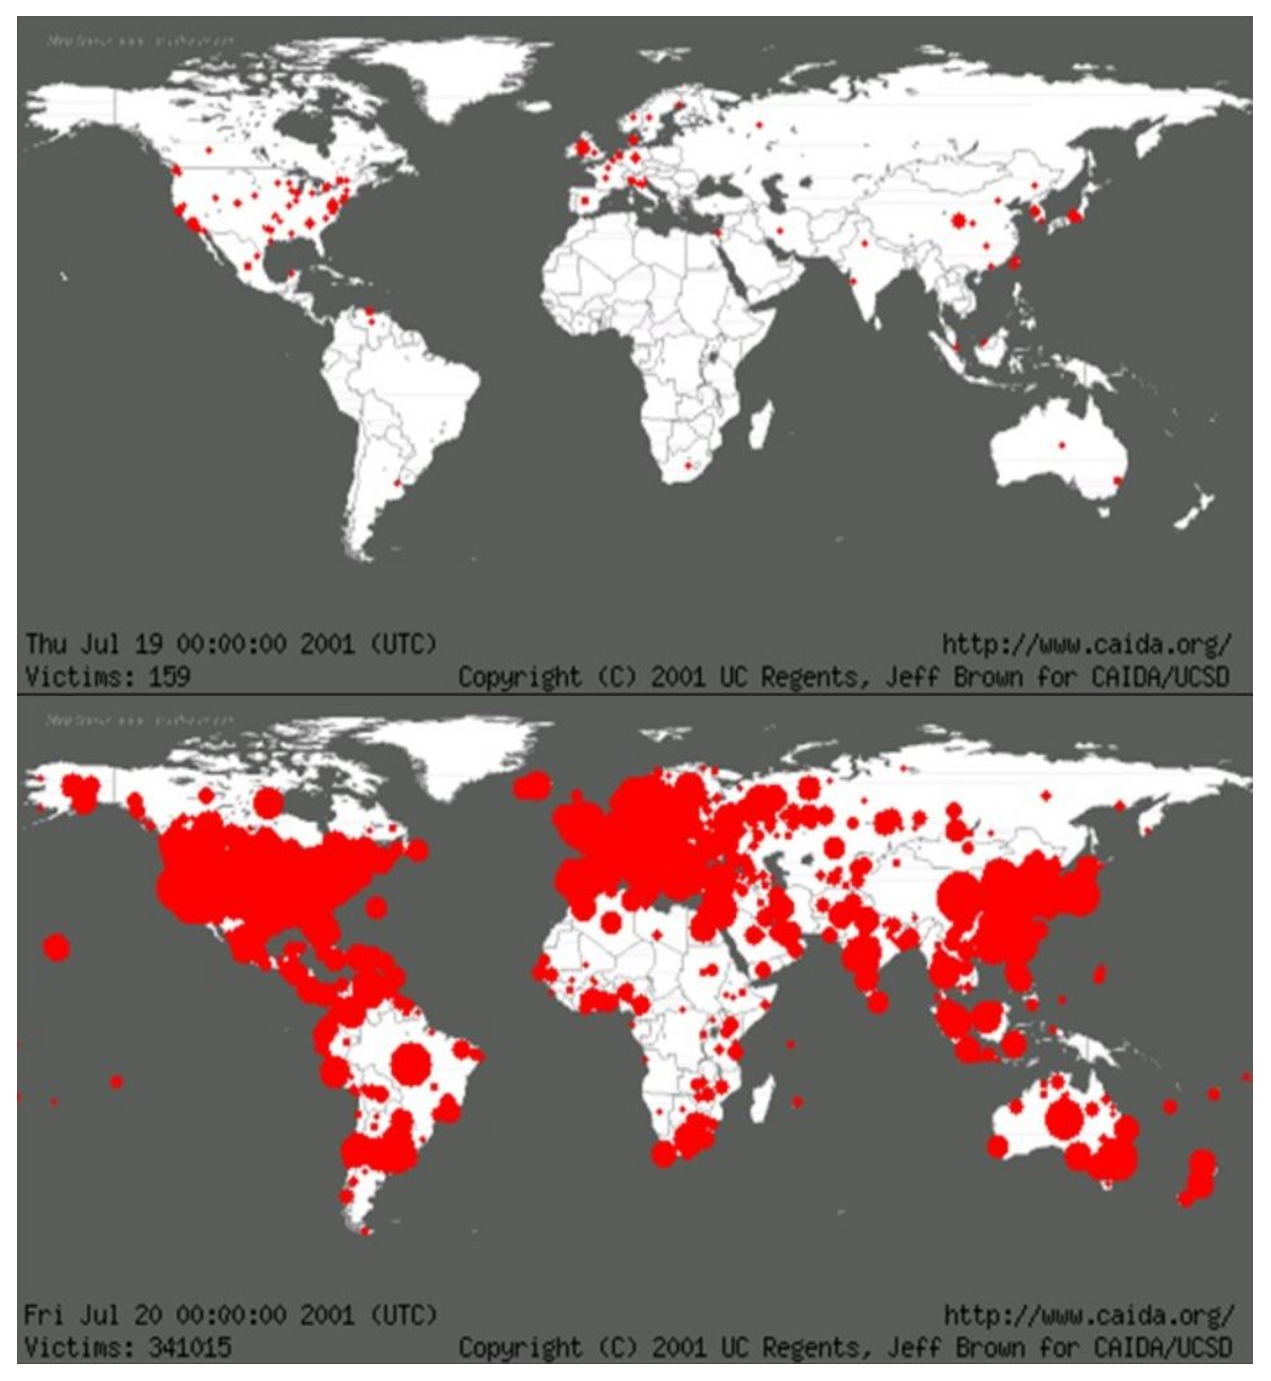
\includegraphics[width=0.8\textwidth]{images/spread.eps}
\caption{diffusione Code Red}
\label{spread}
\end{figure}
Le figure~\ref{infected} e~\ref{rate} danno un’idea del forte impatto che ha avuto la versione di Code Red a seme dinamico, infatti si vede che a partire dalla mattina del 19 Luglio c’è stato un improvviso incremento del tasso di infezione che ha raggiunto un valore di 2000 host al minuto. È interessante notare anche la decrescita esponenziale di tale tasso, dovuta probabilmente al conseguente stato di indisponibilità dei server, all’adozione di contromisure e ai gravi problemi causati alla rete globale che hanno portato ad un inevitabile rallentamento del traffico.\\
\begin{figure}
    \centering
    \begin{minipage}{0.5\textwidth}
        \centering
        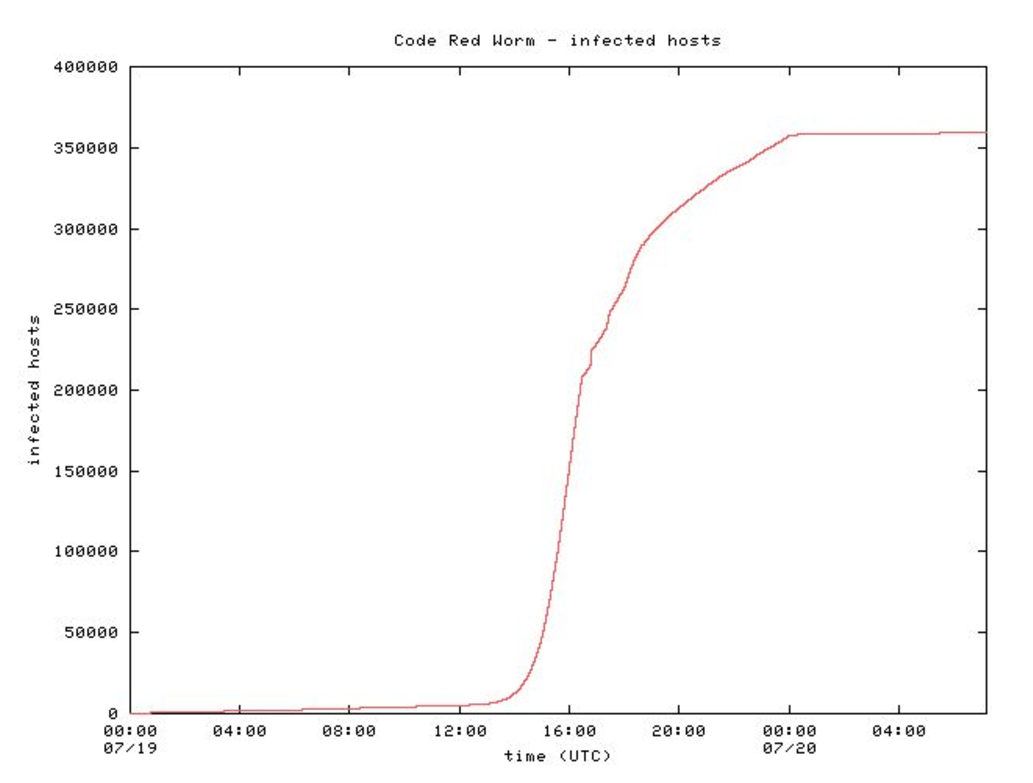
\includegraphics[width=0.95\textwidth]{images/infected} % first figure itself
        \caption{totale host infettati}
        \label{infected}
    \end{minipage}\hfill
    \begin{minipage}{0.5\textwidth}
        \centering
        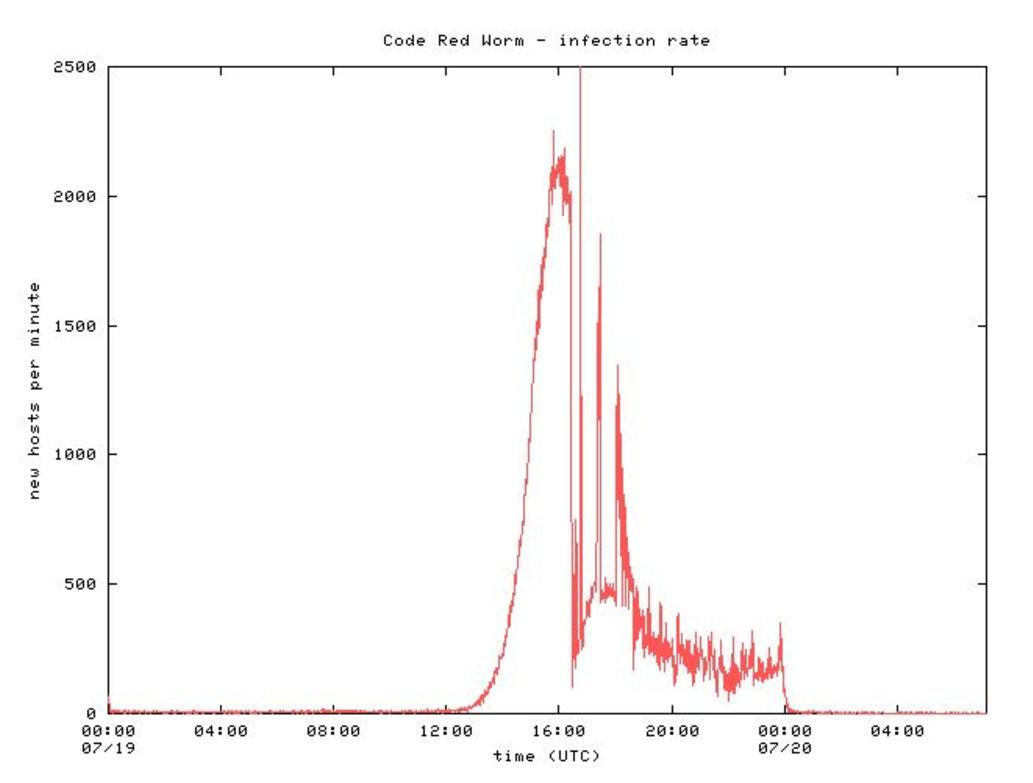
\includegraphics[width=0.95\textwidth]{images/infection_rate} % second figure itself
        \caption{tasso di infezione}
        \label{rate}
    \end{minipage}
\end{figure}
La figura ~\ref{deactivated} mostra il numero di host che hanno smesso di sondare la rete al variare del tempo e, a conferma di quanto detto sopra, tale numero era già pari a circa 200000 unità (oltre il 50\% delle infezioni totali) prima che il worm cessasse definitivamente l’attività di diffusione per procedere alla fase di attacco DDoS.\\
\begin{figure}[!hbp]
\centering
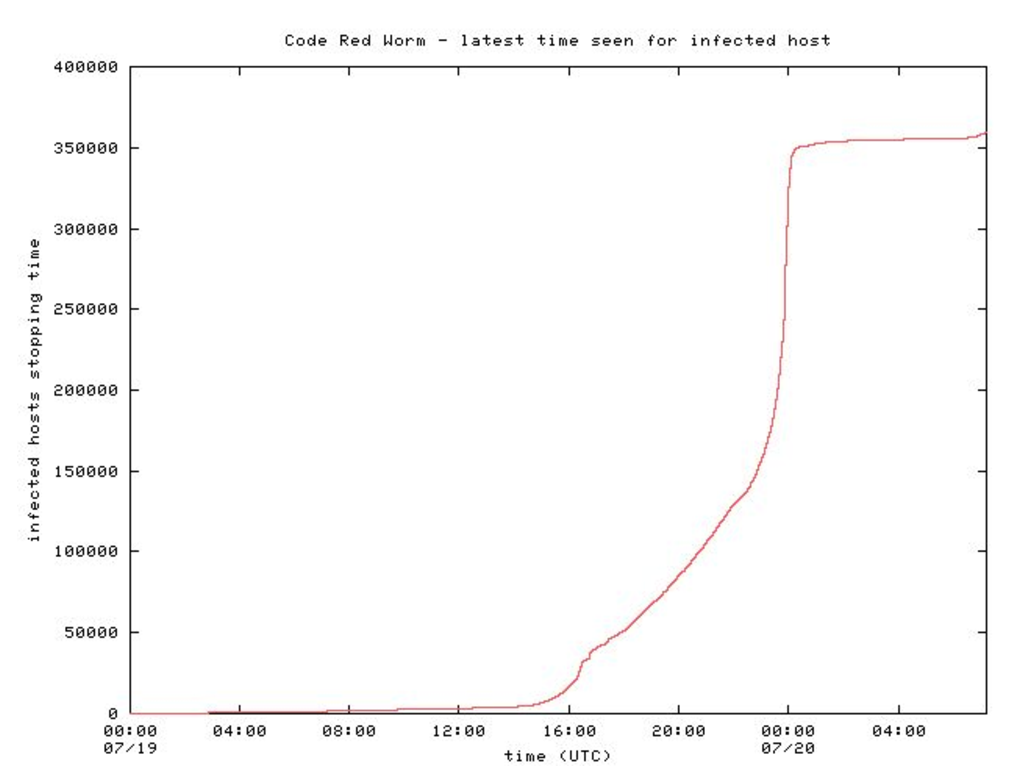
\includegraphics[width=0.7\textwidth]{images/deactivated.eps}
\caption{host "disattivati"}
\label{deactivated}
\end{figure}
Per comprendere la composizione demografica dell’utenza coinvolta, i ricercatori del CAIDA~\cite{caida} hanno esaminato i vari livelli di dominio e la locazione geografica degli host infetti.\\
La figura~\ref{domains} riassume i risultati di tale studio: per quanto riguarda i domini di primo livello la proporzione rispetta la allora attuale situazione dei web server, mentre è curioso notare che il 10\% delle macchine compromesse sono state localizzate in Korea; i principali nomi di dominio sono costituiti da server provider per infrastrutture casalinghe e piccole imprese, da qui si vede che anche queste piccole realtà hanno un ruolo rilevante riguardo la salute globale di internet.\\
\begin{figure}[!hbp]
\centering
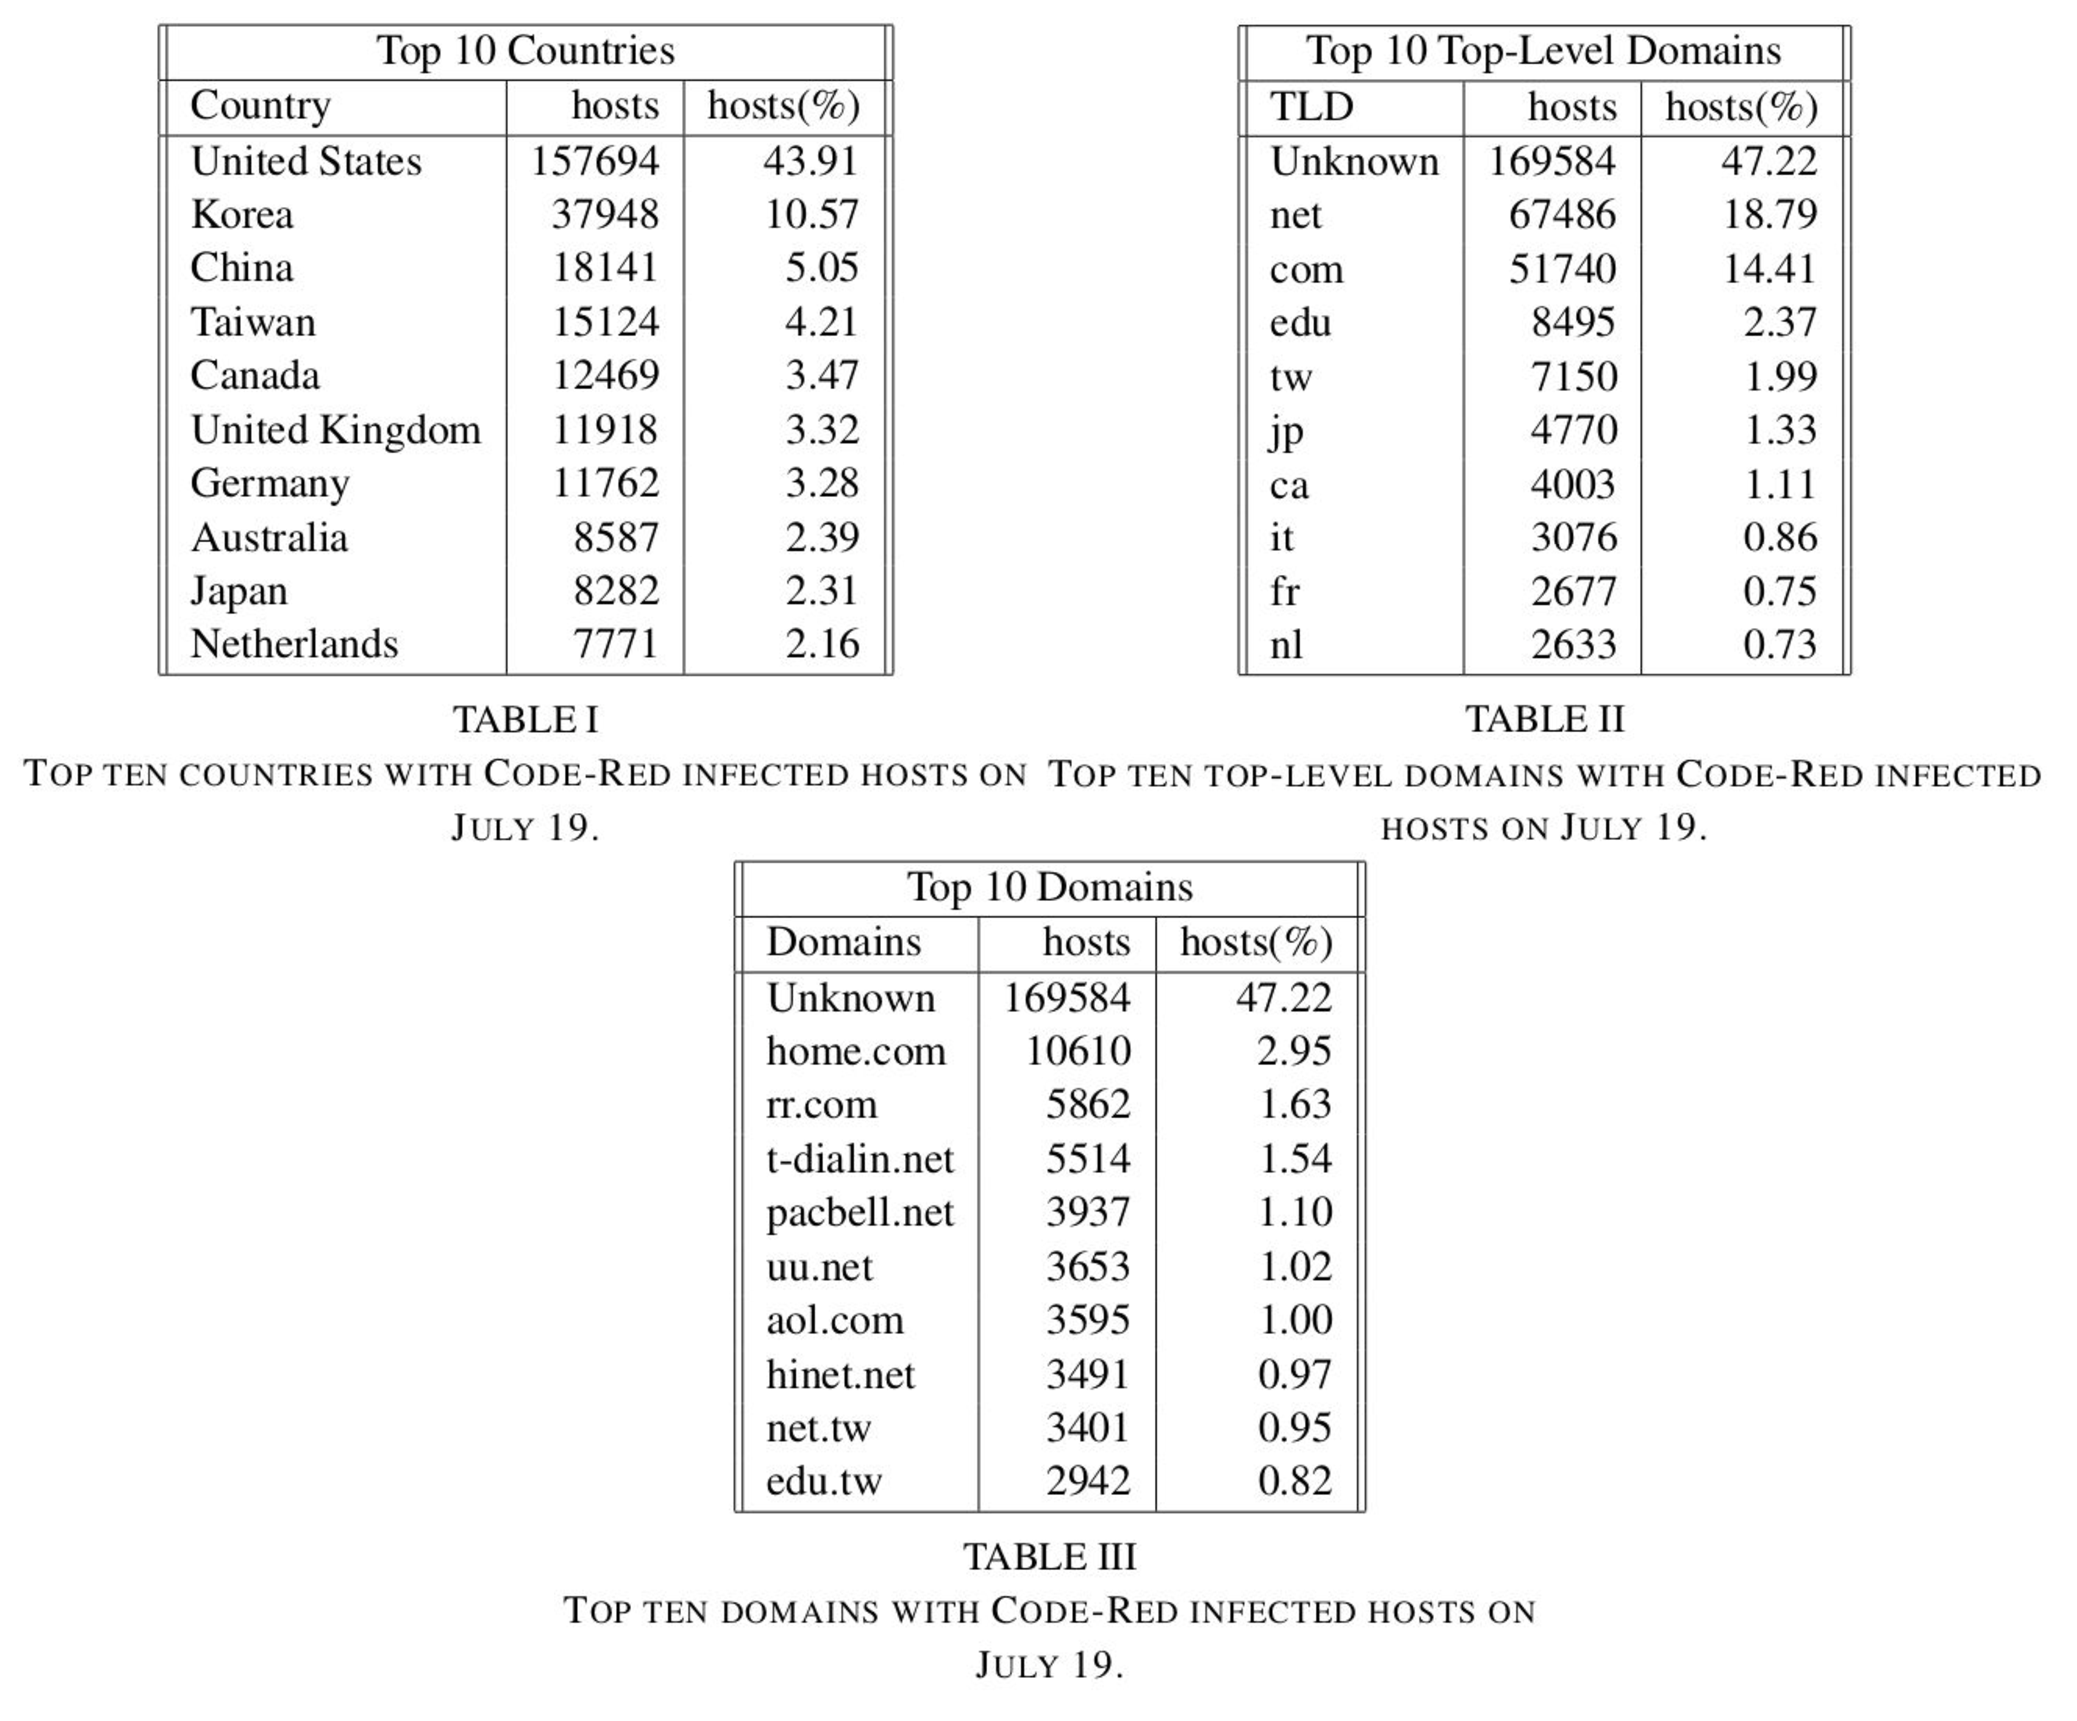
\includegraphics[width=0.8\textwidth]{images/domains.eps}
\caption{risultati analisi demografica}
\label{domains}
\end{figure}
